% Chapter 1

\chapter{Background} % Main chapter title

\label{Chapter2} % For referencing the chapter elsewhere, use \ref{Chapter1} 
\newpage

\section{Advertising}

Everywhere is advertisement of something, some event or a product and it is meant to provide the audience information about those things and gain the planned goals and effects from the specific target audience, it is a mean of mass communication that is created to alter the audience’s behavior and attitude \cite{advertisementdef}. In particular Kotler and Keller defined the advertisement as bellow

\begin{snugshade}
\begin{quote}\textbf{Defination: Advertising }\\ \\ \emph{Advertising is any paid form of non-personal presentation and promotion of ideas, goods, or services by an identified sponsor. Advertisers include not only business firms but also charitable, nonprofit, and government agencies}\end{quote}\cite{ad_def}.
\end{snugshade}

So based on the definition above advertisement is non-personal meaning it is meant to a group of people or target groups, secondly it should represent an idea or basically it should have something to deliver for the people which matters to the audience and normally it does have sponsor(s) to launch it somewhere for example on TV, Radio or print a poster version outdoor. The way message is being delivered has been changing at every era of development as discussed bellow.



\subsection{History of advertisement}
%From very old ages as from 13th century advertising has played an important role to promote customers attention and be able to compete with one another, 
The first paper advertisement was published at 1704 in an American newspaper called Boston News Letter, which was about houses and lands to be sold\footnote{Paper advertisements: http://infoacrs.com/a/adhistory.html, Last accessed 16th March 2016} and after that lots of business started to do their advertisements in newspapers, posters and banners. The first television ad was shown at 1941 on an American TV\footnote {First TV ad: http://www.openculture.com/2013/08/watch-the-first-commercial-ever-shown-on-american-tv-1941.html, Last accessed 16th March 2016}, this ad brought attention to a wide area of application and big business industries toward advertisement as a result the budgets raised much higher for advertisements and later advertisement entered the World Wide Web or so to say online advertising, which has evolved now to multi-billion dollar industry. Now because of the emerging new technologies and advancements, advertisements are in our smart phone applications, smart TV sets, tablet PCs and many other smart devices. And from past decades display screens are replacing print advertisements because of the easy reusability of the screen and convenient usage of them and providing dynamic contents.


\subsection{Traditional Advertising}
Traditional advertising is a form of advertising that uses the media to send commercial messages to the mass audience or viewers, the media can be in any form like TV, Newspaper, Radio, public displays, bill boards and more and in traditional advertising is “the presentation of content is linear and the consumer is passively exposed to product information” \cite{Non_inter_vs_interAd}, user has no control over the flow of the advertisement. 

\subsection{Online advertising}
Online advertising or Internet advertising is a form of advertising that uses email, web, applications, or any internet application used in mobile or computer, that drive direct sales via electronic commerce \cite{onlinead}, as \emph{PWC}  \cite{pwc} researched and there are two trends that give online advertising this boost, (1) increase in webpages, and (2) development in targeted advertising format and beside that there are a lot of ways for online marketing \cite{waysmarketing}, (1) search engine optimization, to suggest websites for users, (2) email, (3) video marketing, like YouTube, (4) Blogging , (5) social media, like Facebook, and many other forms.

\subsection{Pervasive Advertising}
Currently computers play important role in life, and it is becoming nearly common and found everywhere and these computers do not have to be like traditional computers like desktops having keyboard and mouse, it has various forms like it could be our laptop to a smart watch or even a smart pen and these technologies blend in our environments too like different kinds of displays, sensor, security cameras, fridge, washing machine and more, so as a result we have ubiquitous computing environment that is supported by underlying technologies like Internet, middleware and microprocessors, as explained by Mark Weiser \footnote{Ubiquitous Computing: http://www.ubiq.com/hypertext/weiser/UbiHome.html}  \cite{ubiquitous_computing} ``\emph{Ubiquitous computing is the method of enhancing computer use by making many computers available throughout the physical environment, but making them effectively invisible to the user}''. The term pervasive computing is also used instead of ubiquitous  \cite{pervasiv_ubiquitous} and it is constructed from basic elements \cite{pervais_ad} (1) ubiquitous access, (2) context awareness, (3) intelligence and (4) natural interaction and when advertisement is made with the help of pervasive computing which is called ``\emph{pervasive advertising}'' would really help to improve advertisement in general because of the powerful properties of the pervasive computing like ubiquitous feature that computing is integrated seamlessly in environment and it disappears, like as Mark Weiser’s \cite{twenty_first} another central statement was ``\emph{The most profound technologies are those that disappear. They weave themselves into the fabric of everyday life until they are indistinguishable from it}''. Based on above explanation, ``\emph{Pervasive advertising is the use of pervasive computing technologies for advertising purposes.}''\cite{pervasiv_ad}.


\iffalse
\begin{snugshade}
\textbf{Defination: Pervasive Advertising }\\ \\ ``\emph{Pervasive advertising is the use of pervasive computing technologies for advertising purposes.}''\cite{pervasiv_ad}.
\end{snugshade}
\fi

\subsection{Advertising program}
To have and effective and efficient advertising, most big advertising industries follow an advertising program after they have defined the target market and buyer motives, the advertising program is also called as \emph{5Ms} \cite{adprogram}, because it is composed of five steps (1)\emph{Mission},(2) \emph{Money},(3) \emph{Message},(4)\emph{Media},(5) \emph{Measurement}, Figure \ref{fig:adprograme} shows these steps.

\begin{enumerate}

\item \textbf{Mission:} \\
Advertising mission (goal) should come from prior decisions on targeted market and location, this goal can be achieved by a fixed communication process in fix duration between advertiser and audience. There are three advertising goals (1) \emph{Informative Advertising}, it is the early advertising stage, which aims to inform target audience about a product which was not in market before, (2) \emph{Persuasive Advertising}, this happens when there are several competitors of the same product, the advertiser persuades people that their product is the best than others, and (3) \emph{Reminder Advertising}, the need of this type is when a product has been in market from long time like \emph{Coca-Cola} and then there is a need to remind people about that product.

\item \textbf{Money:} \\
Decision on advertising budget is very essential for future of company, the company should clearly invest on the advertising of certain product, if the budget is less then the effect will be less, if the budget is higher it could be also be a risk of overspending.

\item \textbf{Message:} \\
The message of the advertising should be very clear and innovative, and generated in a way that can impact on viewers. It should go from four stages, (1) message generation, (2) message evaluation and selection, (3) message execution and (4) social responsibility review.

\item \textbf{Media:} \\
The media selection is important because it can help to expose the number of desired times an advertisement message to the target audience. The number of exposures of advertisement can define the number of awareness of audience about product. And the effect of exposure depends on, (1)\emph{reach}, how much can the advertiser reach to users, through internet, banners, TV and so on, (2) \emph{Frequency}, How many times that advertisement is going to be shown on those locations, (3)\emph{Impact}, the qualitative value of exposure on audience.
\item \textbf{Measurement:} \\
The last step is to measure how the advertisement was effective, for a specific defined advertisement goal, location, and target audience within a specific duration of time. The measurement will state the level of achievements and what got accomplished and what not.
\end{enumerate}


\begin{figure}[H]
\centering
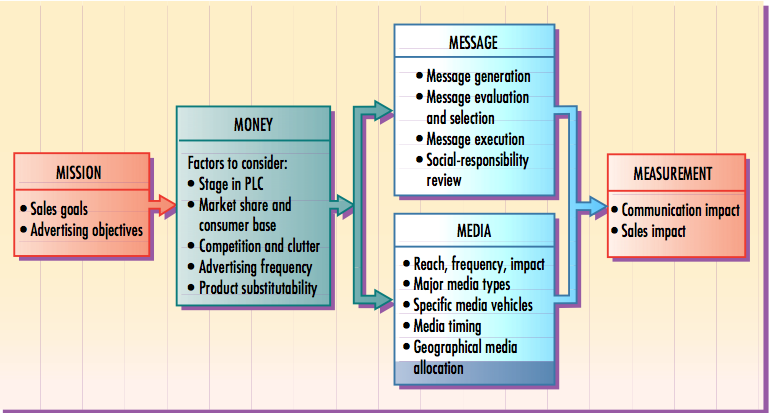
\includegraphics[width=0.9\textwidth,height=90mm]{Figures/2/adprogram}
\caption{Advertising Program, \cite{adprogram}}
\label{fig:adprograme}
\end{figure}




\subsection{Advertisement performance}

Every advertiser is interested in \emph{conversion-rate}, it is ``\emph{the percentage of visitors who take a desired action.}''\cite{convrate}, the desired action is to visit a webpage, buy a product, play a game, or any action which is defined by the advertiser. \emph{conversion-rate} is very important for advertiser to see the efficiency of their advertisements and how to utilize it for mass visitors that could be more effective. In e-commerce, advertisers track user’s each step or click, they track users from search engines to webpages, from webpages to contacts, from contacts to subscribers and from subscribers to \emph{Actions} purchase or downloaded of an application, with the help of a technique called \emph{conversion-funnel} \cite{convfunnel}, all the journey of visitors are described in a funnel like shape, as Saad Kamal \cite{googlefunnel} describes the conversion funnel in Google Analytics, see figure \ref{fig:conversion_funnel} the funnel is composed of four layers, (1) Awareness or attention, (2) interest, (3) Desire and (4) Action, and visitors would have to take these steps to reach the final goal which is purchase of a product. 

\begin{figure}[H]
\centering
\includegraphics[width=100mm,height=80mm]{Figures/2/con-funnel}
\caption{Conversion Funnel}
\label{fig:conversion_funnel}
\end{figure}

The funnel shape shows the decrease of visitors in each layer of funnel, because most visitors may be aware but not interested, and people who are interested are subset of the first layer of funnel, and not all interested people desire to buy a product, so people get decrease in the next layer who desire for a product and may read the details, and specifications, but not all people who desire buy the product because maybe the person does not have money to buy or other reasons, and at the end very few people fit to buy the product and reaches the final layer of funnel (purchase). 
Advertisers can aim different visitors at different layers of conversion funnel, and based on analysis of the funnel advertisers can define where exactly the advertising effort should be invested, \cite{ad_effor_funnel}


The conversion ratio is defined by \emph{click-through rate} (CTR) metric, it is the ratio of the number of clicks on advertisement to the number of visitors who makes impression (see the advertisement) \cite{convfunnel},and advertisers optimize their pages, by analysing that which sections, links of web pages can result in to higher CTR. and to compute the conversion rates the bellow metrics are used.


\begin{itemize}
\item CPM (Cost Per Thousand) \\
It is a benchmarking metric in advertising to calculate the cost of an online advertisement, which defined by showing an ad to thousand of viewers. Advertisers would be charged per impression (thousand of viewers). 

\item CPC (Cost per Click) \\
The advertiser is charged, when a viewer clicks on the advertisement message or link, occasionally it is found in search engines, and famous websites. 

\item CPA (Cost per Action)\\
Advertisers will be charged if the viewer performs an action, the action could be click, register, subscribe, fill a form or any other action.

\end{itemize}





\section{Public displays}
Displays are increasingly getting cheaper and being used in various locations like restaurants, hotels, sport stadiums, homes and now in public space like shop windows, supermarkets, airport and streets and roads. Most of these displays shows advertisement in which dynamic or static content is being shown and at few of them are interactive like purchasing train tickets with a touch capability, checking in airport and even interactive advertisement in which passers-by can be engaged and play game. 
This section discusses on the history of public display, novel applications of display, sensing technologies that are being used in displays, attraction of display and how engagement is designed for displays by the design of novel interaction techniques and at the end how displays are evaluated and what are the methods and tools to do so.


%\begin{snugshade}
%This is based on following publications.
%\end{snugshade}


\subsection{History of public display research}
Various researches have been done from the past three decades and are still continuing until today, as the first research was conducted in 1980 called the ``\emph{Hole-in-Space}'' \footnote{Hole-In-Space: https://www.youtube.com/watch?v=SyIJJr6Ldg8} that connected New York and Los Angeles one side-walk with a live video and sound system, people at both end could hear and see each other, in this research common behavior and interactions of people were explored and other similar researches had also been done.

Different sized displays were also designed to fit working area and space for various tasks, like Mark Weiser illustrated in his paper ``\emph{Computer for 21th century}'' \cite{newgenerationcomputer}, in which he present tabs, pads, and boards devices which could be used as a personal use and also showed large scale displays equivalent to blackboard for public use, and demonstrated that how can these technologies be integrated as ubiquitous and be adjustable based on user demands and context. 

Another research on situated displays that projects content based on location for-example  \emph{FLUMP}\footnote{flexible ubiquitous monitor project: http://research.cs.ncl.ac.uk/cabernet/www.laas.research.ec.org/ \\ cabernet/workshops/radicals/1996/papers/flump-finney.html, last accessed May 15, 2016.} \cite{flump}, this project was designed to research and illustrate the effectiveness and adaptability of ubiquitous computing systems. Many researches also conducted to design wearable displays like Meme tags and group tags \cite{meme-tags} that by wearing the displays participants could share ideas and opinions called “memes-succinct” among themselves, and through large display called “community Mirrors” these memetics exchanges were visualized live for conference audience. Another “Name tags or thinking Tag” from IBM \cite{ibmtags} that would show the name of the person when facing another person and also display relevant information on who is viewing the tag.

Furthermore, ambient displays were also researched for-example the \emph{Waterlamp and the pinwheels} used \emph{ambientRoom} of Ishii and ullmer \cite{ambient}, in which they showed how tangible bits could connect the cyberspace and physical environment and foreground and background of human activities. The room was kind of augmented space using light, sound and airflow and water movement. Another was \emph{office plant\#1} \cite{office_plant}, which was an exploration of a technological object adapted to the office ecology, another was \emph{Information Percolator} \cite{information_precolator}  this ambient display was designed to show expressions placed within decorative objects \footnote{Information Percolator : https://www.youtube.com/watch?v=9LGQWhCePc8, last accessed:16 May 2016},  Greenber and Michael \cite{shared_notes} investigated on how people transition from individual interaction to group work with the use of PDAs and shared displays and based on this they introduced SharedNotes system and illustrated how people can switch to different modes.

Encouraging social interaction was another important aspect for public displays, researchers like Chew and leclerc \cite{chew_interaction} focused conversation in a conference setting using display called \emph{Sparks} which ``\emph{an ambient social networking and communication facilitation interaface}'' this had interactive features on information related to elements presented in the space. Another interactive display designed for hospital \emph{AwareMedia} \cite{ interactive_hospital}, which facilitated  social, spatial, and temporal awareness and supported coordination at an operation ward. Gesture based interactions with ambient display was researched by Daniel Vogel \cite{vogel} that developed interaction framework for sharable, interactive public ambient displays\footnote{Interactive Public ambient display:  https://www.youtube.com/watch?v=aFl71SPeYto, last accessed: 16 May 2016} it could also support implicit and explicit and multi-user interactions, \emph{Blueboard} \cite{blueboard} , which was developed at IBM Research, was a display system for groups to exchange information in a walk-by situation, \emph{IM here} \cite{ imahere} by Elaine M.Haung that researched on LDGAs \footnote{Large display groupware applications} and proposed a design on how to share IM\footnote{Internet messaging} large displays by using mobile phone, this helped to be an awareness and communication tool.

At end of 2000s mobile phones became popular and common among people and was also a good mean of interaction with displays, \emph{C-Blink} \cite{cblink} that used mobile phone display, which was used as light source that sent various hue color to a camera from which the camera would detect and encode information and present on large display. Another approach was the use of Flashlight of phones as a pointing device as Shirazi and winkler \cite{flashlight} described the design of public-private display with flashlight simple interaction. Other features of phone like Bluetooth, Infrared were also used as an interaction mean with display (e.g., \cite{bluetooth2, Bluetooth}).

Consequently advertising also became a focus for researchers as Krüger and Müller illustrated their design of how to recognize passers-by via Bluetooth \cite{toward_situated} and how long did they stood in front of display or whether they read the content or not by video based face detection and by doing this the most relevant information would be presented in the screen, \emph{BlueScreen} \cite{bluescreen} which selected and displayed adverts in response to users detected in the audience,Stepping more further to give users choice of changing and reforming the content shown on display, \emph{Prospero project} \cite{prospero} that developed a display framework that could be configurable and controlled in public, \emph{RunWithUs} \cite{runwithuse} a social sport application that motivated people to do sport and share their progress, \emph{Digifieds} \cite{digifieds} another plateform that users could post ads in public displays.

\subsection{Auto-active displays}
Beside hundreds of researches on public displays, there are other displays, which were and are made by private advertisement industries and most of these displays are auto-active or non-interactive displays, these displays are situated in train station, airports, malls, restaurants and various locations mainly for advertisement purposes. \emph{zipper}\cite{zipper}at year 1928 made LED display at the front corner of the New York Times building, this display was showing current headlines, in Olympic 1979 the very first large display was deployed, which had video enabled \footnote{Olympic glory a short history of Olympic games timing. London in August 2012 \url{http://www.runnersworld.com/olympics/a-short-history-of-the-olympic-games, last accessed:18 May 2016}}, and there are various other companies that until now are working like \emph{printsign} \footnote{printsigne: \url{http://www.printsign.co.uk/}, last access 19 May 19, 2016}, a big company in UK that designs and advertises in big displays for their customers, \emph{Sony Ziris}\footnote{Sony ziris: \url{http://pro.sony.com/bbsc/ssr/cat-monitors/}, last accessed 19 May 2016}, This company sells advertising screen, and supports advertising content to be played on their screens, \emph{BBC big screen}\footnote{BBC big screens: \url{http://www.bbc.co.uk/blogs/aboutthebbc/entries/ea215929-b57e-3bb9-8d01-e0433f93fd62}, last accessed 19 May 2016}, which started at 2013 by installing many of their big screens and shows BBC big live events, and even people who travel by taxi can watch on going advertising and news on go like \emph{taxi TV}\footnote{Taxi TV: \url{http://verifonemedia.com/networks/taxi-media/}}, Another world famous out door advertising company is \emph{ClearChannel} \footnote{\url{http://clearchanneloutdoor.com/}}, \emph{Dynascan}\footnote{ Dynascan: \url{http://www.dynascanusa.com/products/360-degree-led-video-displays/}} is a company that advertises in 360 degree big outdoor and indoor screens, enabled with Content management system that advertisement could be edited, changed,  \emph{Kinton}\footnote{Kinton: \url{http://www.kinoton.de/de/home.html}} another cylindrical LED screen company that supports for big solutions like advertising, cinema and more. 


\subsection{Interactive displays}
Beside auto-active displays, there are a lot of interactive outdoor and indoor displays that is made by private companies, restaurants and some events, \emph{CocaCola}\footnote{Coca Cola Interactive: \url{https://mg337group10.wordpress.com/2015/04/04/coca-cola-and-interactive-advertising/}, last accessed 19 May 2016} is involved to make interactive advertisement in public display, \emph{MC Donald}\footnote{MC Donald Interactive Ad: \url{http://en.nolapeles.com/2011/06/16/mc-donalds-interactive-ad/}, last accessed 19 may 2016} allowed passers-by to connect to the advertisement board and play game and by winning get a coupon number from which he/she could get something for free from MC shop, Other public awareness interactive ads are also there like Interactive Hair-raising awareness\footnote{Hair awareness: \url{https://www.youtube.com/watch?v=qqd6hgO_AOI} last accessed 20 May 2016} an interactive ad that was installed in train station and used ultra-sonic sensor to detect the arrival of train and the model hair was beautifully blown up, Another was an interactive billboard that to let passers-by stop child abuse\footnote{Child Abuse: \url{https://www.dramafever.com/news/powerful-billboard-lets-you-stop-child-abuse-/}, last accessed: 14 May 2016}, Advertisement could be done in various forms and now are in restaurants and bars like Clo Winebar\footnote{17 Awsome bars: \url{http://walyou.com/bars-and-restaurants-themes-geeks/}, last accessed 19 May 2016} a bar that customers are able to view and select orders from an interactive screen, or pizzaHut \footnote{PizzaHut: \url{http://www.fastcocreate.com/3027282/pizza-huts-interactive-touch-table-could-be\\-coming-to-a-restaurant-near-you}, last accessed 19 May 2016} an interactive display that allows customers to design their own pizza and order through it, floor and wall projected interactive advertisement are also common like Aristoz\footnote{Ariztoz: \url{https://www.youtube.com/watch?v=FH2TON7LRIY}, last accessed: 19 May 2016} that illustrates various examples of projection based interactive advertisement in supermarket, hotels and airports, \emph{JCDecaux}\footnote{JCDecaux: http://www.jcdecaux.com/en/, last accessed 19 May 2016} a france famouse advertisement company is booming in innovative outdoor and indoor advertisement, And many more interactive advertisement are out there in public that brings joys and engaging experience to audience.  


\subsection{Engagement with displays}
There is not a single application which would claim to be perfect, it could be good for a specific domain but would lack a lot of things from other perspectives, same applies for public displays that are another mean of communication for passers-by and is more complex than other single user device like mobile phones, There are many layers of complexities that needs to be addressed when dealing with public display, for-example how passers-by be attracted toward display, and when they are attracted how to motivate them toward display to come near and interact and how to design a better interaction medium for the users at that situation, these are all issues that needs to be worked on, Müller et al \cite{DesignSpace} illustrated a model of different interaction phases in which he called it Audience Funnel, as he describes that there are many stages until users actually interact with the advertisement as shown bellow Attention and motivation will eventually lead to interaction and these stages follow each other if the first step fail the rest would not happen, so there is certain thresholds that people should exceed to transition from mode to other, the Audience funnel model was actually based on the model by Brignull and Rogers \cite{ EnticingPeople} in which they researched on social and interactions and behaviors and how to improve them in a way that people do not feel embarrassed or stop them from interactions and engagement. 


\subsubsection{Attention}
Most devices that are being used has an owner and the owner is aware of the device and pays attention to it, for example a mobile phone or a laptop, the owner pays attention and then uses the phone or laptop to do certain task, public displays do not have an owner, or in other words everyone can use them if higher attention is given to them, therefor the job is on displays to be able to provide enough attraction for the passers-by to be engaged. 
Various models of attracting attention have been developed and proposed, Itti and Baldi \cite{attention1} made the bottom-up attention model meaning that the attention could be attracted if a strong external stimuli happen, the model shows various of representation of input image like color, orientation that human brain cells are capable of interpreting them and based on input images the model predicts which area of the picture could have more attention, the model is also equipped by top-down (the brain before shifting attention knows, or has experience to certain regions) processes too.  Florian Alt \cite{pervasiv_ad} stated from previous researches that the attraction attention could be gained by behavioral urgencies and honeypot effect has also strong impact on attracting attention.

Behavioral urgencies models predicts how much a specific external stimuli can gain attention of someone, for example Franconeri and Simons \cite{franconeri} stated that ``\emph{Attention capture is often operationally defined as speeded search performance when an otherwise nonpredictive stimulus happens to be the target of a visual search. That is, if a stimulus captures attention, it should be searched with priority even when it is irrelevant to the task}'', beside this may other things captures attention like sudden appearance of object \cite{capturingattention}.

Honeypot, Brignull and Rogeres \cite{EnticingPeople} describes this effect effect that when ever a bunch of people gather around a display automatically other people are being attracted toward the display. They showed this effect in a party in which they had an interactive system installed called Opinionizer which was a shared display in which people could type their opinion with keyboard and these opinions would be projected in display in a more acceptable way, by doing this people started to notice the messages and most importantly the people taking part, which built an awareness of people toward display. 

\subsubsection{Motivation}
To be motivated means \emph{to be moved to do something}\cite{motiv}, 
Motivation is another big challenge for public displays, passers-by may glance toward display but necessarily not motivated to interact with the display, there is significant need to understand how to motivate passers-by toward display as Thomas \cite{toward_motivation} describes activities that motivates ``\emph{An activity is said to be intrinsically motivated if people engage in it “for its own sake," if they do not engage in the activity in order to receive some external reward such as money or status. I will use the words "fun," "interesting," "captivating," "appealing," and "intrinsically motivating," all more or less interchangeably,}'' he states that challenge, fantasy and curiosity could be categories of motivation instructions.

Challenge is a driving force for motivation, Florian alt \cite{pervasiv_ad} summarizes \emph{Flow}\cite{flow} that state of mind in one sentence by saying ``\emph{is a state of mind where the user is fully immersed in an activity while feeling energized and focused. Simply said, flow can be achieved in a channel between too little challenge (leading to boredom) and too much challenge (leading to anxiety).}'' So there should be balance between them, and to change and interaction to a challenge the end goal should not be clear and known for participants.   

Curiosity happens when something is not so clear, and people tend to find what is actually there, but some may feel insecure to try it because of shy or because of social context, therefore proper explorative behavior is required to overcome these insecurities \cite{motiv}, and to increase curiosity the application should send to the participant a sense of incompleteness and at the mean time should also show how to over come that incompleteness through the use of that application \cite{pervasiv_ad}.

Fantasy is another deriving factor to motivate people toward display, if something imaginary or unrealistic is shown people gives more attention, now with the increasing technologies and computer capabilities, virtual reality, augmented reality and others sensing technologies these fake environments can be built \cite{fantasy_metaphores}, BigBoard \footnote{ https://www.youtube.com/watch?v=UIHwHqaY3SY, last accessed: 19 May 2016} which was installed in a bus station and was showing the video of the side of the bus station and meanwhile was augmenting some fairies coming from sky and approach the participants, by doing this people got motivated and was look the backside to confirm if in reality the fairy exist. JCDecaux\footnote{JCDecaux Innovative ads: https://www.youtube.com/watch?v=Gw0Gfp5LVgQ, last accessed 19 May 2016} creates innovative advertisements which most of them are full of fantasy. 



\subsection{Metaphors}
Advertisements are posted in various forms and there are different mental models categorized by J. Müller \cite{DesignSpace} which are Posters, windows, mirrors and overlays.

\begin{itemize}
\item \textbf{Posters: } \\
From poster definition by Ghosting and peter\cite{Poster_Ad} is ``\emph{A poster is any piece of printed paper designed to be attached to a wall or vertical surface}'', these poster does contain texts, graphics or combination of both and now a days they are not necessarily have to be paper based it could be digital poster that with the use of media like screens a more dynamic contents could be shown. Most of these types of these digital posters show traditional advertising contents but the difference is only being dynamic, which is often ignored by passers-by \cite{display_blindness}, and by integrating sensing technologies these posters could be interactive too to increase the user engagement.


\item \textbf{Windows: } \\
There are advertisements shown at windows facing outside the shop, this type of mental model gives the viewers some sort of clue of a virtual location from one side, but the actual window model should have two sides (this side and remote side) and brings some sort of intercommunication of two sides together, forexample \emph{Hole-in-Space}\cite{hole_space}, which there were two big screens installed in two major cities and live video and audio streams was available for public to communicate 

\item \textbf{Mirrors: } \\
Mirrors are reflective surfaces, displays with mirror model to show the reflection of the passers-by would allow to encourage them for interactions, this is normally done by projecting silhouette representation for example J.Müller \cite{LookingGlass} experimented by mirroring image, silhouette and abstract representation of passers-by.

\item \textbf{Overlays: } \\
Overlays are not bounded to the fixed frame and size like screens or mirrors, they could have various shapes and does not have frames, it could be glass door or a part of a window or a whole wall, the fact is that they can integrate with environment, Normally these are done by using high performance projectors like CLD projector\footnote{LCD projector: http://www.projectorreviews.com/projector-categories/lcd-projectors/, last accessed 19 May 2016}, one of this type of interaction was \emph{Jumping Frog} \cite{ meme-tags}that was projected on surface and by touching it the frog would jump to other surface. 



\end{itemize}



\subsection{Interaction models}
Different interaction models are created as shown bellow that illustrates how passers-by would behave and react at certain regions (zones) toward display, how groups are audience can form and what could be their next step for interaction. 


\begin{enumerate}


\item Hallo.Wall \cite{hello_wall, hellow_wall_2}, which was a context-dependent display reflecting Identity and proximity of passers-by, designed to communicate detailed information, the display was interactive and passers-by could communicate through RFID and WaveLAN technologies though a “distance-dependent Semantic manner” meaning based on different distances various interactions were offered. The interaction model consisted three zones ambient zone, notification zone, and cell interaction zone as can be seen in the picture. 

\begin{figure}[H]
\centering
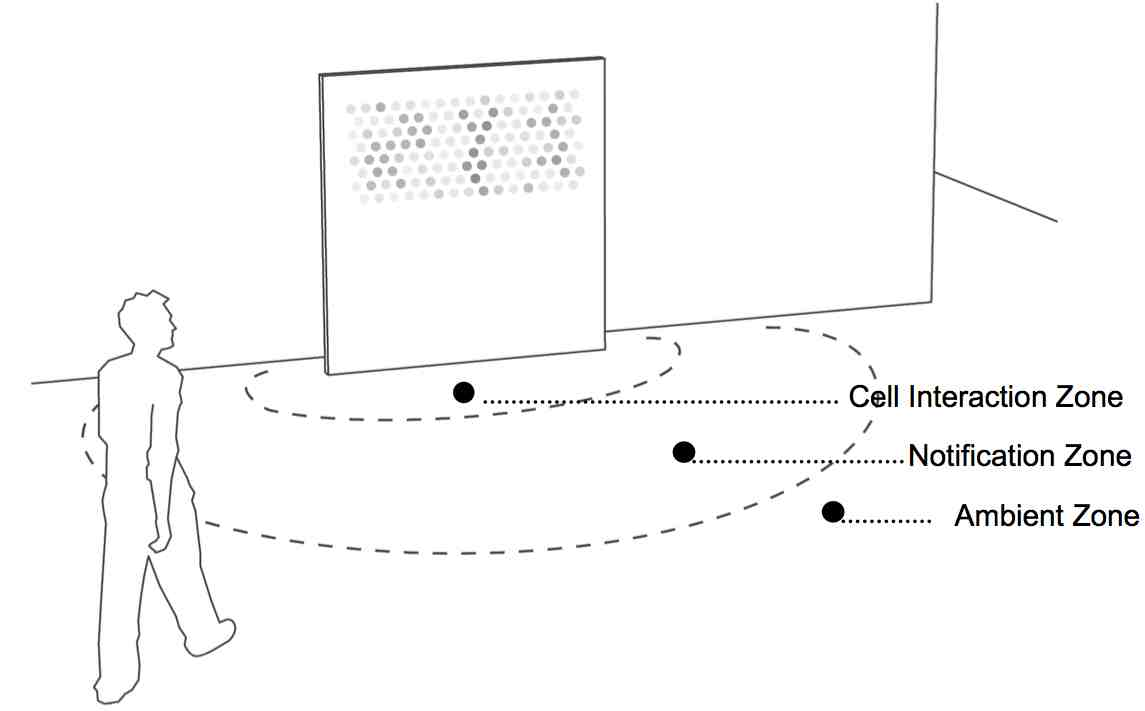
\includegraphics[width=100mm,height=60mm]{Figures/2/hello_wall}
\caption{Three zones of interaction, \cite{hellow_wall_2}}
\label{fig:threezoneofinteraction}
\end{figure}

Ambient zone is outside the sensing area where people cannot be tracked or sensed and passers-by are experiencing ambient mode, in this mode the display shows some information and content independent to the people. Notification zone is the place where is under sensor range and the sensors can detect people and show particular light pattern on the display. Cell interaction zone is the zone, where the passer-by is very near to the screen and can start interacting with display. 


D. Vogel \cite{vogel} used the same interaction design and enhanced that could support transition of implicit to explicit interaction with both personal and public information, He introduced implicit, subtle and personal interaction zones or stages that has smooth transitions in between, as can be seen bellow.


\begin{figure}[H]
\centering
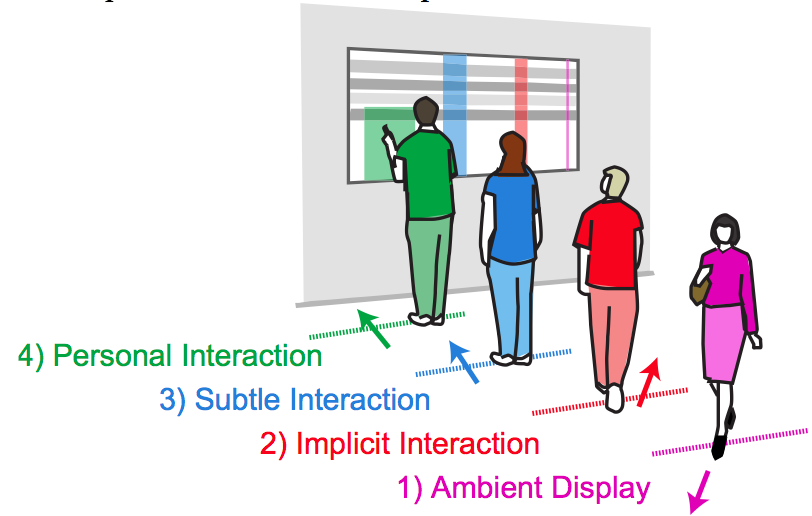
\includegraphics[width=100mm,height=60mm]{Figures/2/hello_wall_refined}
\caption{Four interaction phases, \cite{hellow_wall_2}}
\label{fig:threezoneofinteraction_2}
\end{figure}


Implicit interaction phase the system detects the person information like position orientation and projects notification when user passes, or presents a kind of representation of the person so that the passers-by can see the reaction to be convinced to enter the subtle interaction phase, the subtle mode activates when user give implicit hint like stopping by screen then more detailed notification or state is shown at this point the interaction area is for multiple users too, but when exploring more personal content then the users moves closer to the screen to enable personal interaction phase, in this phase the user is very close to the screen and the interaction could be done by touching the screen and explore more personal contents. 

\item Another interaction model designed by Brignull and Rogers \cite{EnticingPeople} conceptualized an interaction model based on their observation they had done on opinionizer system in a lunch party, and divided the space around display in three categories as space (a) peripheral awareness, space (b) focal awareness and space(c) direct interaction, and illustrated how people switch between these spaces by crossing some thresholds, this model is limited to the interaction medium because on keyboard was used and other phases like implicate and explicit interactions are not considered, and the model is made to be in an environment that people are somehow familiar and standing for long time to know each other which in result removes social embarrassment and people can interact freely with the system instead of ignoring it. 

\begin{figure}[H]
\centering
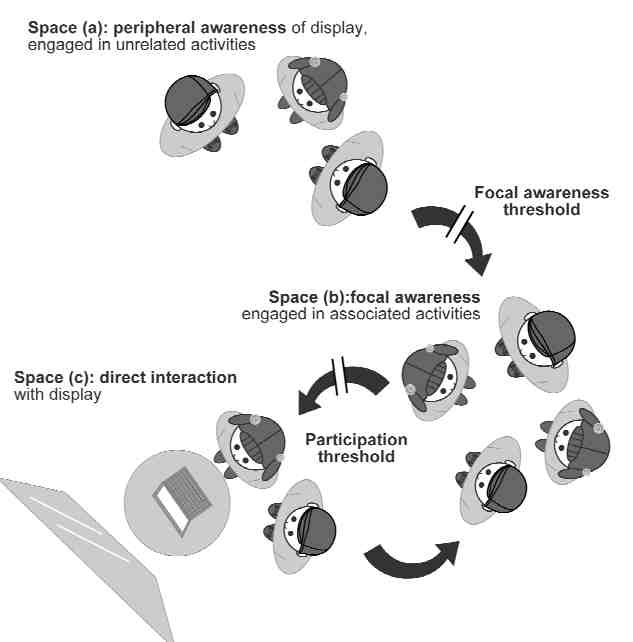
\includegraphics[width=80mm,height=60mm]{Figures/2/opinionizer}
\caption{A diagram of public interaction flow accross thresholds, \cite{EnticingPeople}}
\label{fig:opinionizerphases}
\end{figure}

\item \emph{Audience funnel} \cite{AudienceFunnel} is another design based on public interaction flow model that have several interaction phases and the phases shows a linear process type in which first should happen then next happens, the phases are  passing by, viewing / reacting, subtle interaction, direct interaction, multiple interaction, and follow-up actions as shown in bellow diagram. This type of model is very interesting for advertising applications.


\begin{figure}[H]
\centering
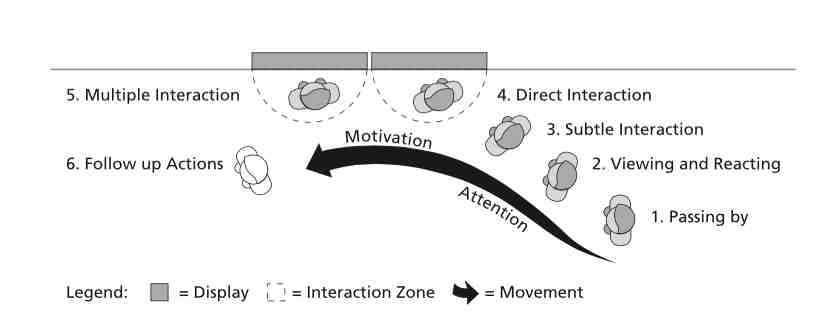
\includegraphics[width=120mm,height=60mm]{Figures/2/TheAudienceFunnel}
\caption{The Audience Funnel, \cite{AudienceFunnel}}
\label{fig:audience_funnel}
\end{figure}

\end{enumerate}



\subsection{Technologies}
The driving force for all these designs and concepts and advancements are the technologies behind them, without the use to advanced technologies it would have not been possible to implement and evaluate the prototypes and designs. This section explores various technologies used for different purposes as listed bellow.


\begin{itemize}

\item Displays: \\
Currently four technologies are used in displays 

\begin{itemize}
\item CRT (Cathode Ray Tube), which was invented by German physicist Ferdinand Braun\footnote{Ferdinand Brown: 
http://www.britannica.com/biography/Ferdinand-Braun, last accessed 21 May 2016} in 1897 that has three electronic guns (Red, Green, Blue phosphor dots) and high speed electrons  from these guns hit the flat fluorescent screen line by line by which the image is created on the screen.  

\item LCD (Liquid crystal display), which is widely used in in Television sets and other computer screens, and has almost replaced CRT, it uses Light-modulating properties of liquid crystal\footnote{Liquid Crystal: https://en.wikipedia.org/wiki/Liquid\_crystal, last access 21 may 2016},which does not shot light rays, to show images. 

\item PDP (Plasma display panels), unlike LCD display is free of distortions if seen from sides, uses tiny neon light for each pixels in the screen and that illuminates the pixels and is designed to display both analog and digital computer inputs\footnote{PDP: http://whatis.techtarget.com/definition/plasma-display}.

\item OLED (Organic Light-Emitting Diode) this technology uses light emitting diodes, that allow for higher resolution and screen size, is one of the expensive displays and has wide viewing angle, better power consumption,


\item There are various other display technologies used for different purposes and screen sizes as listed bellow.

\begin{itemize}
\item E Ink (Electronic paper)
\item PDP (Plasma display panel)
\item ELD (Electroluminescent display)
\item DMS (Digital microshutter)
\item ...

\end{itemize}

\end{itemize}

\item Sensors: \\
Now technology is highly advancing and day-by-day new sensors for different purposes are being made, and the sensors which in past was difficult to use because of many dependencies and had cost a lot of money is now easy to use with very limited requirements and less price. Sensors are listed based on their purposes as bellow.


\begin{itemize}

\item \textbf{Presense} \\
Presence is the state or fact of being present as with others or in a place\footnote{Presence: http://www.dictionary.com/browse/presence}, there are sensors that can sense if someone is at the proximity or vicinity of the display and can even sense how far the person is in meter or centimeter in relation to display. 


\begin{itemize}
\item Cameras: \\
Now there are many cheap and powerful cameras that has integrated firmware that does Human tracking capabilities so easy for example Mircrosoft Kinect Camera\footnote{Microsoft Kinect: \url{https://developer.microsoft.com/de-de/windows/kinect}, Last accessed: 1/05/2016 at 13:21:00}, which comes in two versions Kinect xbox360(V1) and Kinect One (V2) these cameras can sense the location of the person, other cameras could also be used and computer vision applications to do track people. 

\item Audio sensors\footnote{Audio sensors: https://www.sparkfun.com/categories/186, last accessed 22 may 2016}: \\
The use of microphones allow us to track sound frequencies and source of sounds originating and from which the distance can be estimated.

\item Audio sensors\footnote{Audio sensors: https://www.sparkfun.com/categories/186, last accessed 22 may 2016}:\\
The use of microphones allow us to track sound frequencies and source of sounds originating and from which the distance can be estimated.

\item Bluetooth: \\
Mobile phones that have enabled Bluetooth can be detected near display.  

\item IR (Infrared): \\
 this could be used to sense the people around as it was used in MemeTags \cite{meme-tags}

\item RFID (Radio-Frequency Identification):\\
RFID serves the same as bar code it can be attached at backside of card, this technology could be used to sense if there is someone near display.


\end{itemize}


\item \textbf{Body position and Posture}
Body position can be detected with pressure sensors installed on the ground floor this would accurately detect the exact coordinate, and beside that Camera can also detect exact position like Kinect camera. Body posture is the orientation of body where actually the body is facing to; this can be detected using 3D Camera or motion tracking. 

\item \textbf{Getures}
Gesture gives more control to the system while interaction, it could be used for manipulating some objects on the screen or control elements, there are many technologies that recognize gestures, like touch screens, accelerometer, and most widely used now is the use of camera in which the user hand or eye or different body posture can be used as some sort of gestures. 

\item \textbf{Touch}
There are various touch technologies available, the use of touch technology evolved from smart phone like iPhone, and spread to screens, Now mobile screen can support multi-touch and screens beside multi-touch can even support multi-user multi touch, touch could be sensed by the display directly or by IR camera that uses computer vision software to track users finger.

\end{itemize}

\item WiFi 
WiFi allows computers, smartphones, tablets or other personal smart devices to connect to private LAN (Local Area Network) or Internet, the use of this technology has become very frequent and almost all handheld devices has the capability to connect, By using this technology people can connect to public displays and interact by using some applications or web controllers. 

\end{itemize}


